\documentclass[conference]{IEEEtran}
\IEEEoverridecommandlockouts
% The preceding line is only needed to identify funding in the first footnote. If that is unneeded, please comment it out.
\usepackage{cite}
\usepackage{url}
\usepackage[english]{babel}
\usepackage{amsmath,amssymb,amsfonts}
\usepackage{algorithmic}
\usepackage{graphicx}
\graphicspath{ {./images/} }
\usepackage{textcomp}
\usepackage{xcolor}
\def\BibTeX{{\rm B\kern-.05em{\sc i\kern-.025em b}\kern-.08em
    T\kern-.1667em\lower.7ex\hbox{E}\kern-.125emX}}
\begin{document}

\title{Free-viewpoint video synthesis for soccer games\\
% {\footnotesize \textsuperscript{*}Note: Sub-titles are not captured in Xplore and
% should not be used}
% \thanks{Identify applicable funding agency here. If none, delete this.}
}

\author{\IEEEauthorblockN{Davide Lusuardi}
\IEEEauthorblockA{\textit{Department of information engineering and computer science} \\
\textit{University of Trento}\\
Trento, Italy \\
davide.lusuardi@studenti.unitn.it}
}

\maketitle

\begin{abstract}
This paper presents some methods for free viewpoint synthesis that generate novel views of actions from any angle and 
allows viewers to virtually fly through real soccer scenes.

% In this document, we discuss some methods to accomplish free-viewpoint video visualization for soccer scenes.
% These methods generate novel views of actions from any angle and allow viewers to virtually fly through real soccer scenes.
% TODO: complete
% and is of interest for visualization in TV productions.
\end{abstract}

% \begin{IEEEkeywords}
% component, formatting, style, styling, insert
% \end{IEEEkeywords}

\section{Introduction}
Nowadays, sport broadcasting plays a large role in current society.
Therefore, it is important to provide a high quality and visually pleasing reporting of sports events.
One common issue in sports is that incidents tend to be over very quickly.
Slow-motion replays can be used to illustrate these incidents as clearly as possible to the viewer. 
Although time is stretched in these replays, there is no exploration of the spatial scene information, which is 
usually important for understanding the event.
A system that allows a replay from any angle adds a lot of value to the viewer experience.

% Especially sports broadcast-
% ing is a well-known recreational aspect of television.
% Therefore, it is important to provide a high quality and
% visually pleasing reporting of sports events.

% In sport most interesting incidents tend to be over very quickly.
% A system that allows a replay from any angle adds a lot of
% value to the production of sport coverage. Sports producers
% may use techniques such as slow-motion replays to illustrate
% these incidents as clearly as possible for the viewer. Although
% time is stretched in these replays, there is no exploration of
% the spatial scene information, which is usually important for
% understanding the event.

Free-viewpoint video (FVV) is one of the recent trends in the development of advanced visual media type
that provides an immersive user experience and interactivity when viewing
visual media. Compared with traditional fixed-viewpoint
video, it allows users to select a viewpoint interactively and
is capable of rendering a new view from a novel viewpoint \cite{05_plane_sweeping}.
Examples of physically impossible camera views which
could be desirable are the goal keepers view, a player tracking camera or even a
ball camera.
% Since a virtualized reality system that distributes 51
% cameras over a 5 m done with controlled lighting and well-calibrated
% cameras was introduced, 
FVV has been a research topic in the field of computer vision 
since a virtualized reality system was developed \cite{04_fast_FVV_01},
ranging from static models for studio applications with a fixed
capture volume, controlled illumination, and backgrounds \cite{02_iview} 
to dynamic object models for sports scenes.
Live outdoor sports such as soccer involve several additional challenges for both acquisition and processing 
phases. 
The action take place over an entire pitch and video acquisition should be done at sufficient resolution in order to
do analysis and production of desired virtual camera views.

% TODO: si può aggiungere questo...
% Moreover, this has not been confined to academia,
% the companies LiberoVision, Intel, and 4DViews also attach
% importance to the technique and have been providing visual
% effects applications for various purposes.

In this paper we briefly present and compare the following methods to accomplish free-viewpoint video 
visualization for soccer scenes: the \textit{iview} system \cite{02_iview}, where automatic online camera calibration, 
segmentation and 3D reconstruction is performed;
the work of Goorts et al. \cite{05_plane_sweeping}, where a plane-sweep approach is used; 
and the work of Ohta et al. \cite{03_billboard}, where a billboard-based representation is employed to simplify the 
3D model.


% TODO: aggiungere da qualche parte
% There is a demand from the broadcast industry for more flexible production tech-
% nologies at live events such as sports. The ability to place virtual
% cameras at any location around or on the pitch is highly attractive to broadcasters
% greatly increasing flexibility in production and enabling novel delivery formats such
% as mobile TV. Examples of the type of physically impossible camera views which
% could be desirable are the goal keepers view, a player tracking camera or even a
% ball camera.

\section{Overview}
In the field of computer vision, the techniques for synthesizing virtual view images from a number of real camera
images have been studied since the 1990s.
% Free-viewpoint video in soccer TV broadcast
% production 
% The requirements for free-viewpoint video in sports TV broadcast
% production
Free-viewpoint video in sports TV broadcast production is a challenging problem involving the conflicting requirements of 
broadcast picture quality with video-rate generation.
FVV techniques for generating novel viewpoints using a multiview camera setup can be categorized into two classes 
\cite{05_plane_sweeping}: 3D reconstruction and image-based rendering. 

Using 3D reconstruction, it is possible to construct 3D models of objects that provides a geometric proxy which can be
used to combine observations from multiple views in order to render images from an arbitrary viewpoint. 
Several approaches have been realized for reconstruction: visual-hull, photo-hull, stereo, and 
global shape optimisation \cite{02_iview}.
% TODO: si può scrivere di più da 02
The quality of the virtual view image generated
by these methods depends on the accuracy of the 3D model. In order to produce an accurate model, a
large number of video cameras surrounding the object should be used. 
Although 3D reconstruction is robust, artifacts such as ghosting objects can be introduced if a lot of objects are in the scene. 

Image-based methods generate the image of the novel viewpoint directly without explicitly reconstructing the 3D scene structure.
The quality of rendered views depends on the accuracy of alignment between multiple view observations 
\cite{05_plane_sweeping,02_iview}.
Usually, these methods are limited to rendering viewpoints between the camera views.
% In many
% methods, depth generation, implicit or explicit, is
% done concurrently.



% Moreover, ... TODO:01
% Furthermore,
% camera calibration [13] is usually required to relate 2-D co-
% ordinates in images to their corresponding 3-D coordinates in
% object space. As it is essential to measure the 3-D positions of
% several points in the object space, calibration becomes difficult
% especially in a large space. For these reasons, the object area is
% generally limited to a few cubic meters in this approach.

% TODO: overview dei sistemi esistenti presente in 02


\section{The iview system}
In this section we present the DTI-funded collaborative project \textit{iview} \cite{iview_project},
a free-viewpoint video system which enables the production of novel desirable camera views.
This system exploits the already placed live TV broadcast cameras as the primary
source of multiple view video.
Usually, football matches are covered by 12-20 high-definition cameras placed all over in the stadium
providing wide-baseline views.
Match cameras are manually controlled to follow the game play zooming in on events when occurs.
However, only a fraction of these are focused on specific events of interest and can be used for production 
of free-viewpoint renders, the remaining cameras cover the pitch, crowd and coaches.


% Robust algorithms are required for both recovery of camera
% calibration from the broadcast footage and wide-baseline correspondence between
% views for reconstruction or view interpolation.

% Therefore
% iview uses a method for real-time camera calibration from the match footage [2:46].
% Player segmentation is performed using chroma-key and difference matting tech-
% niques independently for each camera view [2:15]. Automatic calibration and player
% segmentation for moving broadcast cameras results in errors of the order of 1-3
% pixels which is often comparable to the size of players arms and legs in the broad-
% cast footage. Robust reconstruction and rendering of novel viewpoints is achieved in
% the iview system by an initial conservative visual-hull reconstruction followed by a
% view-dependent refinement. View-dependent refinement simultaneously refines the
% player reconstruction and segmentation exploiting visual cues from multiple cam-
% era views. This achieves free-viewpoint rendering with pixel accurate alignment of
% neighbouring views to render novel views with a visual quality approaching that
% of the source video.

% Advances are presented in real-time through the
% lens camera calibration to estimate both the camera pose, focus and lens distortion
% from the pitch marks.

% Free-viewpoint video is then produced starting with a volu-
% metric reconstruction followed by a view-dependent refinement using information
% from multiple views.

% Automatic online calibration, segmentation and reconstruction is performed to allow
% rendering of novel viewpoints from the moving match cameras.

\begin{figure}[htbp]
\centerline{\includegraphics[scale=0.078]{iview_overview2.png}}
\caption{Overview of the free-viewpoint system. [TODO: cite 02.1]}
\label{fig:iview_overview}
\end{figure}


The \textit{iview} system is composed of three main modules as shown in Figure \ref{fig:iview_overview}: 
capture, processing and replay module.

Capture is performed using time synchronised acquisition from both auxiliary and
match cameras.
The minimal number of cameras is about four, but for good quality results a higher number is required.
Camera synchronisation is achieved using standard genlock process.

The processing module computes a 3D model of the scene.
This is done using segmentation of objects from the back-
ground and 3D reconstruction \cite{2.1_iview}.

In order to allow the use of footage from match cameras and to avoid the need for prior calibration, 
automatic calibration of all cameras is performed using a line-based approach againts the pitch lines of the captured footage, 
achieving a root-mean-square error of 1-2 pixels for moving cameras. 
The calibration is very fast and robust, capable of real-time operation for use during live match footage. 
Calibration estimates the extrinsic and intrinsic parameters of each camera including lens distortion.

The segmentation is needed to separate the foreground, i.e. the players from the background.
Matting of players from the green pitch is performed using chroma-keying matting. 
% This allows the approximate segmentation of the foreground players for subsequent processing to produce free-viewpoint video. 
The authors developed and tested a k-nearest neighbour approach for chroma-keying and evaluated two other known techniques,
\textit{Fast green subtraction} in RGB colour space and keying in HSV colour space.
The k-nearest neighbour classifier is controlled by a GUI where the user has to click on position in the image that corresponds
to the background. 
The process is repeated until the resulting segmentation is satisfying.
A deeper explanation is present in the paper \cite{2.1_iview} where the authors present and evaluate also 
\textit{Fast green subtraction} and keying in HSV.

The accumulation of errors from calibration and matting can cause large errors in
the reconstruction of the scene, such as loss of limbs. 
Therefore, robust algorithms have been developed for scene reconstruction.
One possible technique is called visual-hull (VH) and represents the maximum volume occupied by an object
given a set of silhouettes from multiple views \cite{2.2_iview_08}.
The visual-hull is a single global representation integrating silhouette information from all
views. A polygonal mesh surface is typically extracted and texture mapped by resampling
the captured multiple view video for rendering \cite{2.2_iview}.
Due to accumulating errors in camera calibration and segmentation, visual-hull accuracy is reduced.
A refinement of the view-dependent visual hull (VDVH) \cite{2.1_iview_12}
using stereo correspondence to interpolate between captured
views can be used to overcome these issues achieving the best alignment between adjacent views and 
hence improve visual quality.
More information about \textit{iview} 3D reconstruction can be found in \cite{02_iview,2.1_iview,2.2_iview}.

Finally, the replay module renders the novel view of the scene using the computed 3D model together with the
original camera images.
Cameras closer to the virtual viewpoint are chosen to generate the novel viewpoint.
% TODO: può essere descritto maggiormente the replay module 


The method proposed achieves an image quality comparable to that of the input images and it is robust to the
wide-baseline moving camera views at different resolutions.
Calibration and segmentation are very important in order to obtain an overall good quality of the system.
Degradation in image quality will also occur if there are insufficients views for reconstruction.
% TODO: si può aggiungere contenuto

% Aperture correction is also applied to each video sequence to correct for the camera edge enhancement
% used in standard broadcast footage \cite{iview}.

% Likewise matting in relatively uncontrolled outdoor conditions with changing illu-
% mination achieves a segmentation within 1-2 pixels of the true foreground with the
% addition of background clutter for the crowd, hoardings and on-pitch advertising.





% The replay module renders the captured scene in realtime
% using the computed 3D model and the original camera images
% deploying view-dependent texture mapping [8].
% The entire system can potentially operate in real-time. At
% the current stage the processing is done offline. That means
% the images are stored and the processing is run at a later stage.
% The replay module is designed to work at interactive rates.
\section{Image-based rendering}

\begin{figure}[htbp]
\centerline{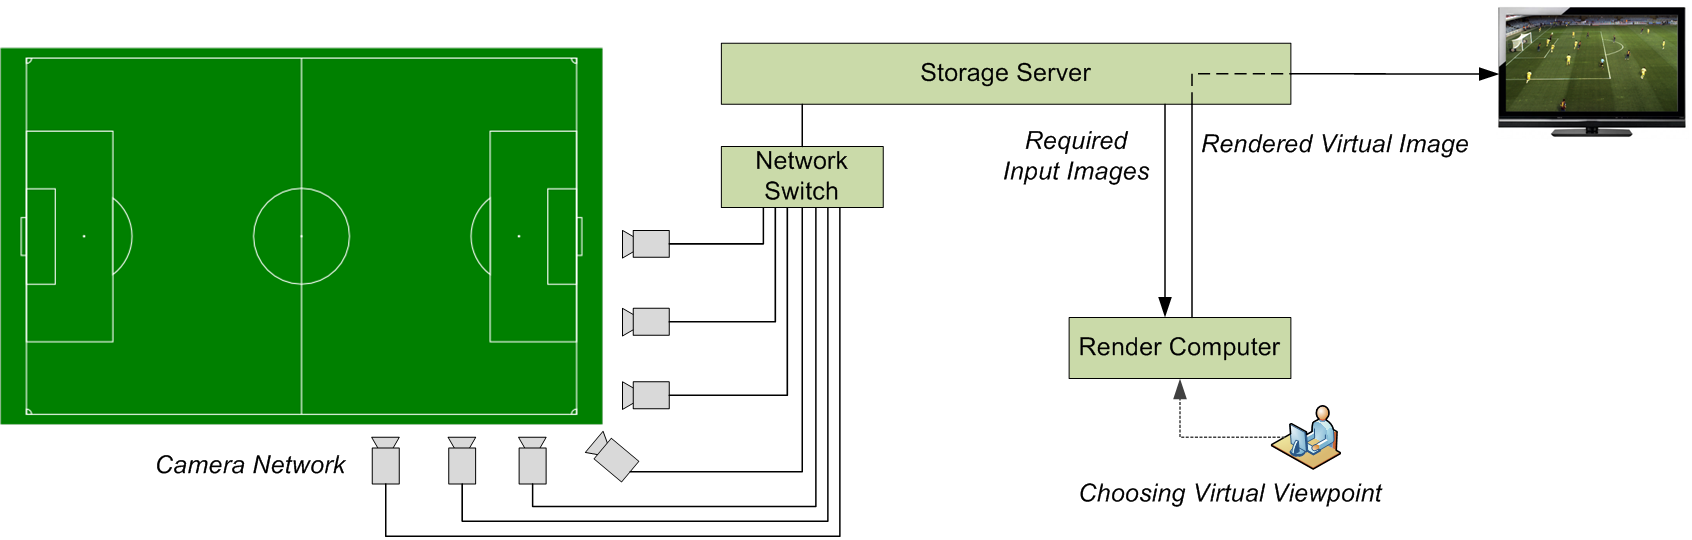
\includegraphics[scale=0.078]{plane_sweeping.png}}
\caption{Overview of the free-viewpoint system. [TODO: cite 02.1]}
\label{fig:plane_sweeping}
\end{figure}

In this section we present a different approach to FVV.
Instead of performing 3D reconstruction, image-based methods generate directly the image of the novel viewpoint.
When multiple cameras are present, plane sweeping can be used [05:Yang et al., 2004] for both small and wide 
baseline setups.
Plane sweeping has already been used for novel view point in soccer scenes. Goorts et al. [05:Goorts
et al., 2012a; Goorts et al., 2013a] present a method
with two plane sweeps and a depth filtering step suitable for smaller baseline 
setups of about 1 meter. 
Moreover, this method has some problems like disappearing players
if they overlap in the image.


\section{Billboard-based visualization}
In this section we present the work of Ohta et al. \cite{03_billboard}.
The authors use billboard representation to make a 3D model of each player.
This method is simpler than full 3D reconstruction and require less computation.
A player billboard is a small rectangle standing perpendicular to the ground
and a 2D texture is shown on it.
The difference between 3D reconstruction and billboard representation is shown in Figure \ref{fig:billboard_comparison}:
as we can see, the visual difference is clear at a close viewpoint but becomes very small at a distant one.
For this reason, becomes particularly important to place player billboards at a right place and direction.

\begin{figure}[htbp]
\centerline{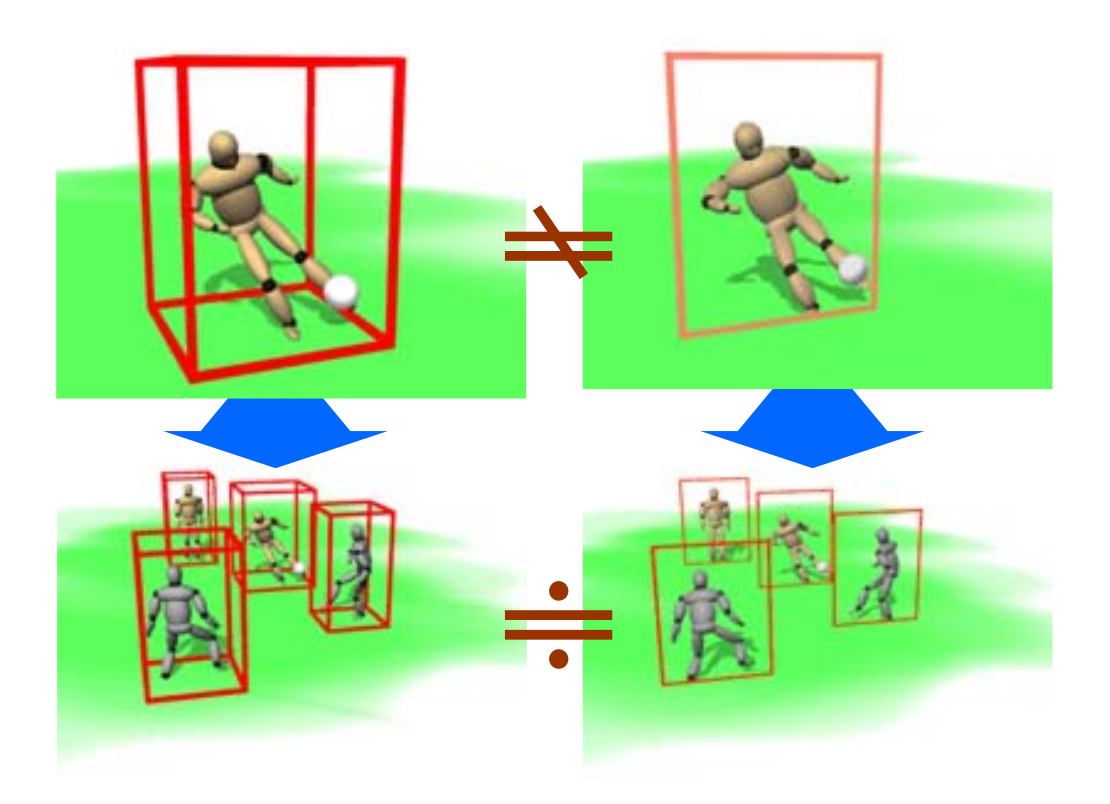
\includegraphics[scale=0.22]{billboard_comparison.png}}
\caption{Appearance similarity between 3D reconstruction and billboard in close and distant view \cite{03_billboard}.}
\label{fig:billboard_comparison}
\end{figure}


The system proceeds as follow: first extracts texture segments from camera videos, then selects appropriate textures according
to the virtual viewpoint and finally layouts the player billboards in virtual space.

Texture extraction phase consists in obtaining the location of each player and extracting texture segments from every image 
video by projecting player location onto the image plane.
Background region is removed in the texture by video capturing PC.
Please note that camera calibration is done before this phase.

Texture selection phase selects a set of texture to be sent to each viewer based on his viewpoint. 
Given a viewpoint, the system finds the camera that minimizes the angle between the line from the viewpoint to the player 
location and the line from the camera to the player location. Then, a texture segment obtained by that camera is selected 
and placed so that the texture face the viewpoint \cite{03_billboard}.
% TODO: completare


One possible problem happens when players are overlapped each other at a certain camera and billboard texture could include both
players.
To eliminate extra player region, authors used stereo based method \cite{03_billboard_04} as explained in \cite{03_billboard}. 
% TODO: can be explained more



\section{Conclusion}
We have briefly presented three free-viewpoint systems for soccer games: the \textit{iview} system, an image-based method using 
plane sweeping, and a billboard-based method.

The \textit{iview} system is a robust method using a multi-camera setup that performs 3D reconstruction exploiting a refinement 
of the view-dependent visual hull method.
% This method requires % TODO: finire

The image-based method presented interpolates real camera images using a plane sweeping approach.
High quality images using wide baseline setup are obtained and typical artifacts are removed.

The billboard-based method is simpler than full 3D reconstruction and requires less computation.
However, this method produces lower quality images, and some visual artifacts can be present.





\bibliographystyle{IEEEtran}
\bibliography{biblio.bib}



\end{document}